%%%%%%%%%%%%%%%%%%%%%%%%%%%%%%%%%%%%%%%%%
% Beamer Presentation
% LaTeX Template
% Version 1.0 (10/11/12)
%
% This template has been downloaded from:
% http://www.LaTeXTemplates.com
%
% License:
% CC BY-NC-SA 3.0 (http://creativecommons.org/licenses/by-nc-sa/3.0/)
%
%%%%%%%%%%%%%%%%%%%%%%%%%%%%%%%%%%%%%%%%%

%----------------------------------------------------------------------------------------
%	PACKAGES AND THEMES
%----------------------------------------------------------------------------------------

\documentclass{beamer}

\mode<presentation> {

% The Beamer class comes with a number of default slide themes
% which change the colors and layouts of slides. Below this is a list
% of all the themes, uncomment each in turn to see what they look like.

%\usetheme{default}
%\usetheme{AnnArbor}
%\usetheme{Antibes}
%\usetheme{Bergen}
%\usetheme{Berkeley}
\usetheme{Berlin}
%\usetheme{Boadilla}
%\usetheme{CambridgeUS}
%\usetheme{Copenhagen}
%\usetheme{Darmstadt}
%\usetheme{Dresden}
%\usetheme{Frankfurt}
%\usetheme{Goettingen}
%\usetheme{Hannover}
%\usetheme{Ilmenau}
%\usetheme{JuanLesPins}
%\usetheme{Luebeck}
%\usetheme{Madrid}
%\usetheme{Malmoe}
%\usetheme{Marburg}
%\usetheme{Montpellier}
%\usetheme{PaloAlto}
%\usetheme{Pittsburgh}
%\usetheme{Rochester}
%\usetheme{Singapore}
%\usetheme{Szeged}
%\usetheme{Warsaw}

% As well as themes, the Beamer class has a number of color themes
% for any slide theme. Uncomment each of these in turn to see how it
% changes the colors of your current slide theme.

%\usecolortheme{albatross}
%\usecolortheme{beaver}
%\usecolortheme{beetle}
%\usecolortheme{crane}
%\usecolortheme{dolphin}
%\usecolortheme{dove}
%\usecolortheme{fly}
%\usecolortheme{lily}
%\usecolortheme{orchid}
%\usecolortheme{rose}
%\usecolortheme{seagull}
%\usecolortheme{seahorse}
%\usecolortheme{whale}
%\usecolortheme{wolverine}

%\setbeamertemplate{footline} % To remove the footer line in all slides uncomment this line
%\setbeamertemplate{footline}[page number] % To replace the footer line in all slides with a simple slide count uncomment this line

%\setbeamertemplate{navigation symbols}{} % To remove the navigation symbols from the bottom of all slides uncomment this line
}

\usepackage{graphicx} % Allows including images
\usepackage{booktabs} % Allows the use of \toprule, \midrule and \bottomrule in tables
\usepackage[utf8]{inputenc}
\usepackage[spanish]{babel}
\usepackage{amsmath}
\usepackage{amssymb}
\usepackage{amsfonts}
\usepackage{listing}
\usepackage{xcolor}
\usepackage[numbered,framed]{matlab-prettifier}
\lstset{
  style              = Matlab-editor,
  basicstyle         = \mlttfamily,
  escapechar         = ",
  mlshowsectionrules = true,
}
%----------------------------------------------------------------------------------------
%	TITLE PAGE
%----------------------------------------------------------------------------------------

\title[Otsu2D]{Segmentación de imagenes mediante Otsu con información espacial} % The short title appears at the bottom of every slide, the full title is only on the title page

\author{Iñigo Biedma} % Your name
\institute[UPNA] % Your institution as it will appear on the bottom of every slide, may be shorthand to save space
{
Visión Artificial \\ % Your institution for the title page
\medskip
Semestre Otoño 2015
}
\date{15 de enero de 2016} % Date, can be changed to a custom date

\begin{document}

\begin{frame}
\titlepage % Print the title page as the first slide
\end{frame}

\begin{frame}
\frametitle{Contenidos} % Table of contents slide, comment this block out to remove it
\tableofcontents % Throughout your presentation, if you choose to use \section{} and \subsection{} commands, these will automatically be printed on this slide as an overview of your presentation
\end{frame}
%----------------------------------------------------------------------------------------
%	PRESENTATION SLIDES
%----------------------------------------------------------------------------------------

%------------------------------------------------
\section{Información espacial e Histograma2D} % Sections can be created in order to organize your presentation into discrete blocks, all sections and subsections are automatically printed in the table of contents as an overview of the talk
%------------------------------------------------

\begin{frame}
\begin{columns}[c]
\column{.45\textwidth}
\begin{align*} 
\frac{1}{n^2}\begin{pmatrix}
 a_{11} & \cdots & a_{1n}\\ 
 \vdots & \ddots & \vdots\\ 
 a_{n1} & \cdots & a_{nn}
 \end{pmatrix}\\
 \forall i,j\ a_{ij}=1
\end{align*}

\column{.6\textwidth}
Tomaremos la media de los valores de gris en la vecindad de cada píxel como información espacial.

\end{columns}
\end{frame}

\begin{frame}
\begin{columns}[t] % The "c" option specifies centered vertical alignment while the "t" option is used for top vertical alignment
\column{.45\textwidth} % Left column and width
\begin{figure}
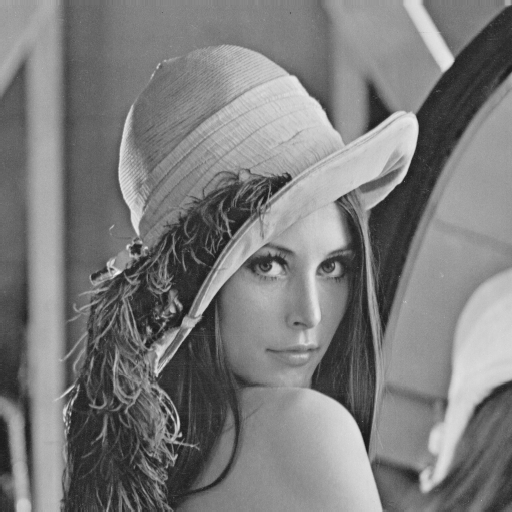
\includegraphics[width=\textwidth]{../../Semestre5/VA_Practicas/Otsu2D/Entrega/lena512.png}
\caption{lena512 original}
\end{figure}

\column{.45\textwidth} % Right column and width
\begin{figure}
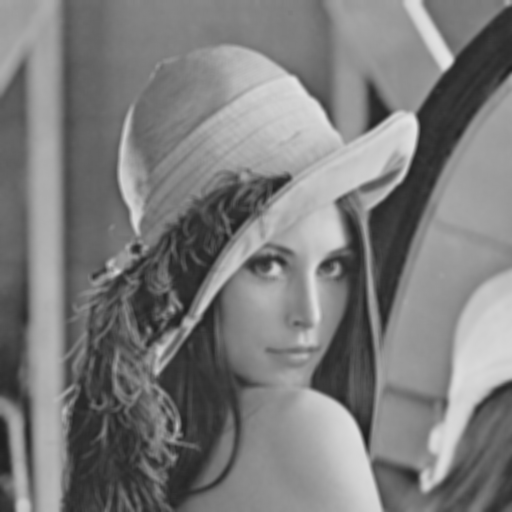
\includegraphics[width=\textwidth]{../../Semestre5/VA_Practicas/Otsu2D/Entrega/lena512s.png}
\caption{matriz de medias de lena512}
\end{figure}

\end{columns}
\end{frame}

\begin{frame}
\frametitle{El Histograma}
\begin{columns}[c] % The "c" option specifies centered vertical alignment while the "t" option is used for top vertical alignment
\column{.4\textwidth} % Left column and width
\begin{figure}
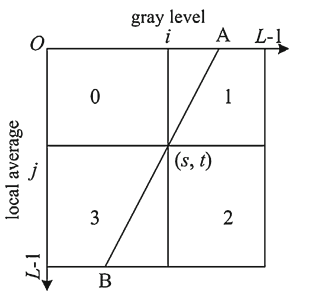
\includegraphics[width=\textwidth]{../../Semestre5/VA_Practicas/Otsu2D/Entrega/graylevel1.png}
\caption{Histograma \cite{p1}}
\end{figure}

\column{.6\textwidth} % Right column and width
En el histograma guardaremos información de los niveles de gris y de las medias locales. En cada valor $(s,t)$ tendremos el número de píxeles de intensidad $s$ cuya vecindad tiene un nivel de gris $t$. 

\end{columns}
\end{frame}

%------------------------------------------------
\begin{frame}
\begin{figure}
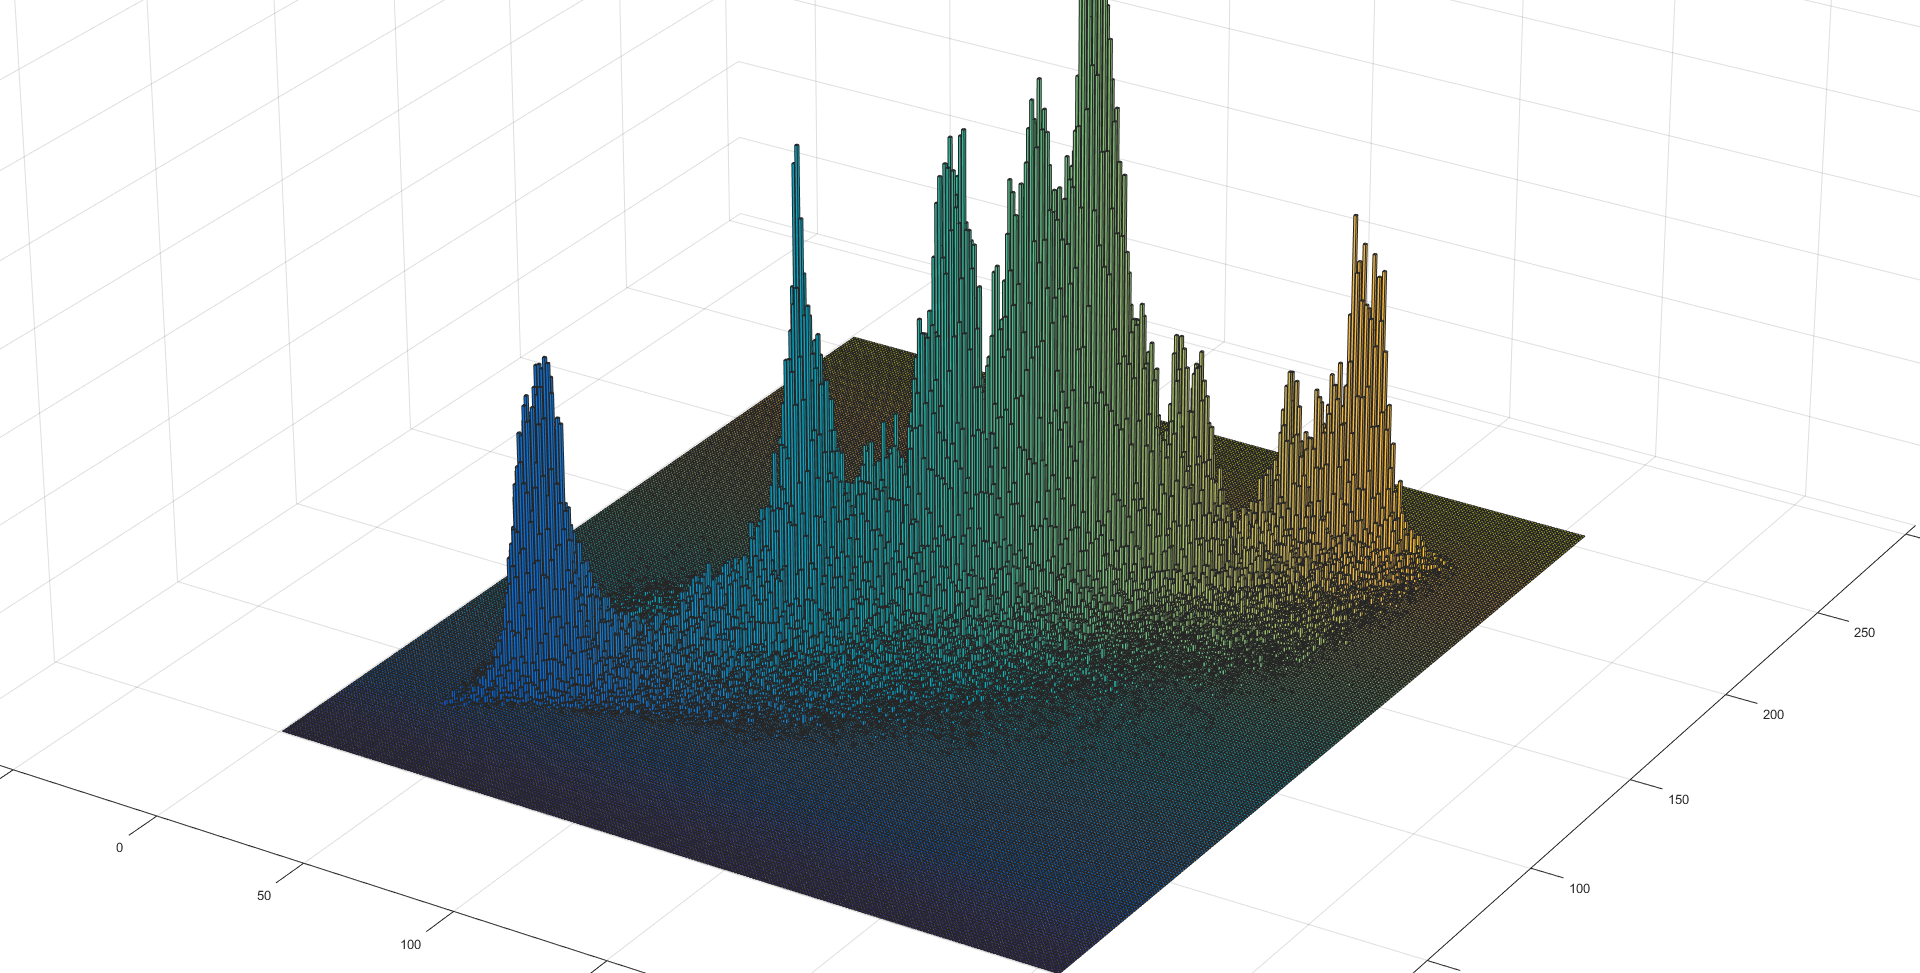
\includegraphics[width=\textwidth]{../../Semestre5/VA_Practicas/Otsu2D/Entrega/2dbar_lena.png}
\caption{Histograma de lena512}
\end{figure}
\end{frame}
%------------------------------------------------

\begin{frame}
\frametitle{Sobre el histograma}
\begin{itemize}
\item La mayor parte de la información está en la diagonal
\item Los cuadrantes 1 y 3 se suelen ignorar. Contienen los pixeles de ruido y los bordes.
\item En el algoritmo Otsu2D básico sólo tenemos en cuenta los cuadrantes 0 y 2
\item Podemos estar perdiendo información
\end{itemize}
Por ejemplo, un píxel de ruido dentro del objeto. Tiene un valor de gris diferente al del objeto pero su vecindad nos permite saber que pertenece.
\end{frame}

%------------------------------------------------

\begin{frame}
Ruido impulsivo
\begin{columns}[t] % The "c" option specifies centered vertical alignment while the "t" option is used for top vertical alignment
\column{0.8\textwidth} % Left column and width
\begin{figure}
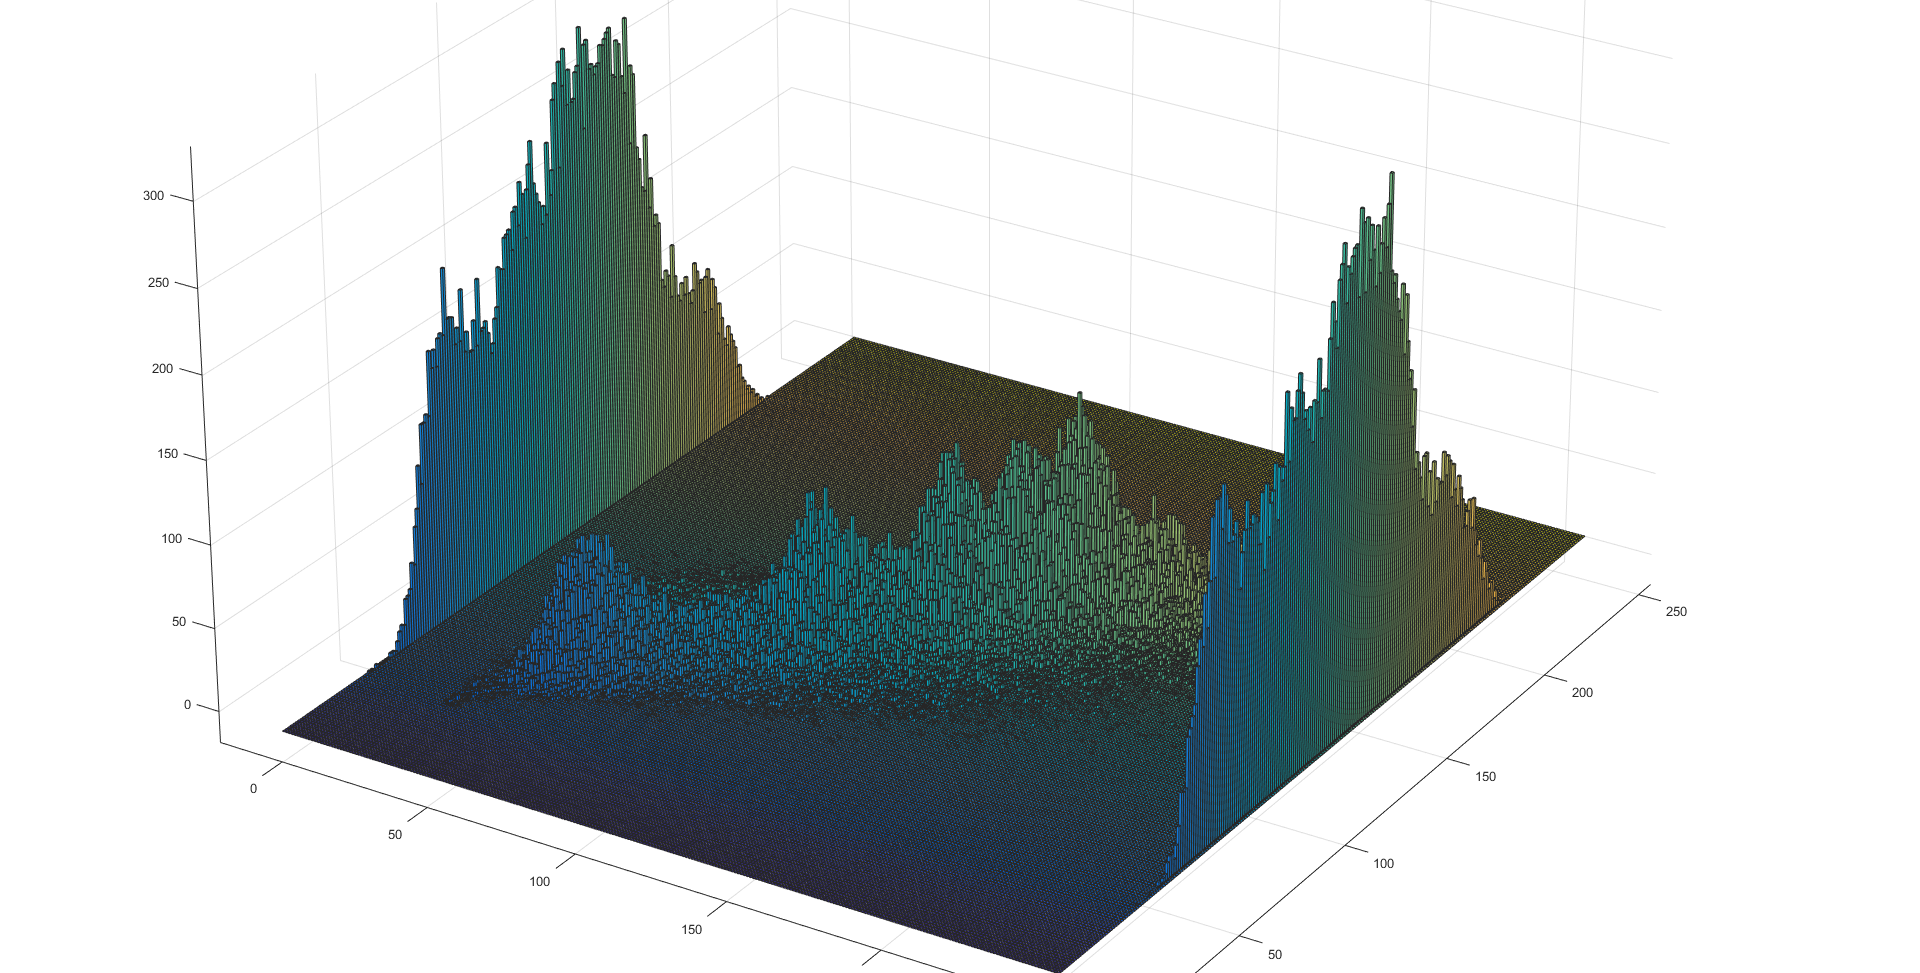
\includegraphics[width=\textwidth]{../../Semestre5/VA_Practicas/Otsu2D/Entrega/2dbar_lenasp20.png}

\end{figure}

\column{.3\textwidth} % Right column and width
\begin{figure}
\includegraphics[width=\textwidth]{../../Semestre5/VA_Practicas/Otsu2D/Entrega/lena512sp20.png}
\end{figure}

\end{columns}
\end{frame}

\begin{frame}
Ruido gaussiano
\begin{columns}[t] % The "c" option specifies centered vertical alignment while the "t" option is used for top vertical alignment
\column{0.8\textwidth} % Left column and width
\begin{figure}
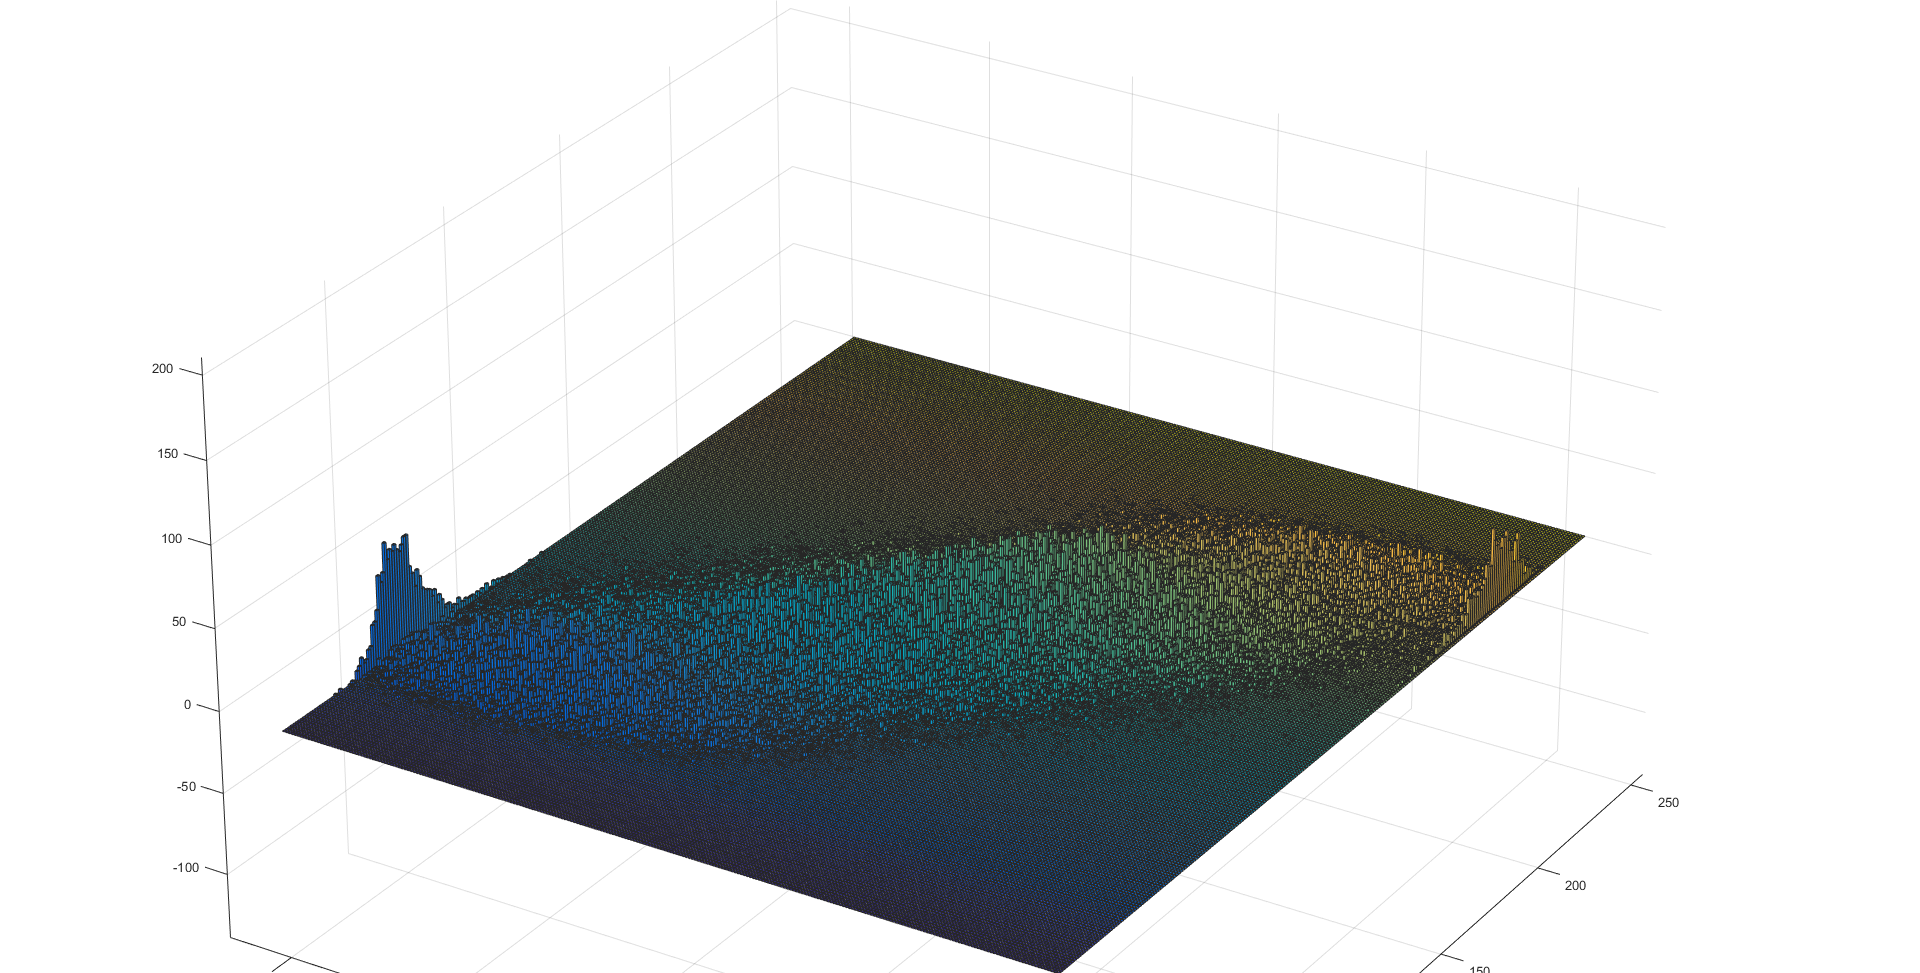
\includegraphics[width=\textwidth]{../../Semestre5/VA_Practicas/Otsu2D/Entrega/2dbar_lenag.png}

\end{figure}

\column{.3\textwidth} % Right column and width
\begin{figure}
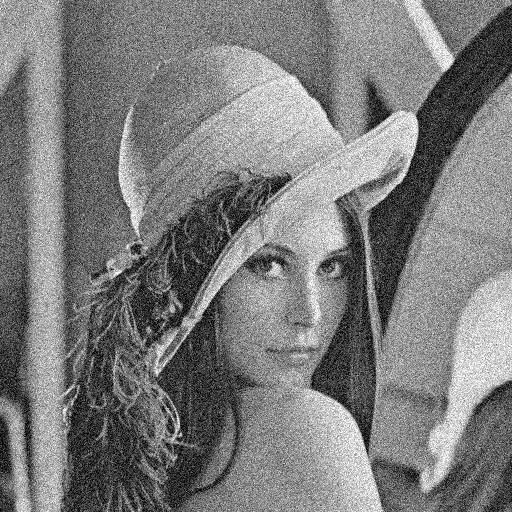
\includegraphics[width=\textwidth]{../../Semestre5/VA_Practicas/Otsu2D/Entrega/lena512g.png}
\end{figure}

\end{columns}
\end{frame}

%------------------------------------------------
\section{Tratamiento del Histograma}
%------------------------------------------------
\begin{frame}
\frametitle{Los métodos}
El procedimiento básico y los dos métodos propuestos. En el básico se toma solo información de los cuadrantes de la diagonal.\\
En todos los métodos \textbf{se busca obtener un histograma en una única dimensión para después clasificar por regiones}.
\begin{columns}[t] % The "c" option specifies centered vertical alignment while the "t" option is used for top vertical alignment
\column{0.6\textwidth} % Left column and width
\begin{figure}
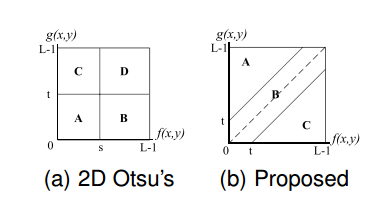
\includegraphics[width=\textwidth]{../../Semestre5/VA_Practicas/Otsu2D/Entrega/metodo2.png}

\end{figure}

\column{.6\textwidth} % Right column and width
\begin{figure}
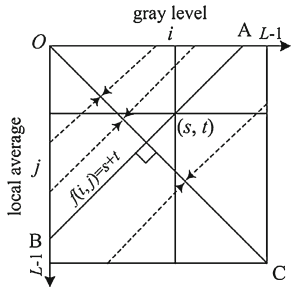
\includegraphics[width=0.5\textwidth]{../../Semestre5/VA_Practicas/Otsu2D/Entrega/metodo1.png}
\end{figure}

\end{columns}
\end{frame}

\begin{frame}
\frametitle{Primer método}
\begin{itemize}
\item Se aplica el gradiente al histograma y se aplica Otsu para separar el histograma en 3 regiones. 
\item De la region B se tienen en cuenta sus valores de gris y no los de su vecindad 
\item De las regiones A y C se toman la informacion de la region pero no sus valores de gris
\item Se aplica Otsu de nuevo al histograma ponderado de esta manera
\end{itemize}
\end{frame}

\begin{frame}
\frametitle{Segundo método}
\begin{itemize}
\item Buscamos la recta que separe el histograma en dos regiones: Objeto y fondo
\item Como hay muchas rectas tendremos solo en cuenta las perpendiculares a la diagonal.
\item Cada recta tendrá una aportación en el nuevo histograma
\item Se aplica Otsu de nuevo al histograma
\end{itemize}
Este es el algoritmo implementado
\end{frame}
%------------------------------------------------
\section{Clasificación}
%------------------------------------------------
\begin{frame}
\frametitle{Las rectas}
\begin{columns}[t] % The "c" option specifies centered vertical alignment while the "t" option is used for top vertical alignment
\column{.6\textwidth} % Left column and width
Las rectas perpendiculares a la diagonal $OC$ siguen la ecuación $f(i,j)=s+t$\\
Tendremos $2L-1$ rectas\\
De cada recta tomaremos la suma de sus valores:
$$p_r = \sum_{f(i,j)=s+t}{h_{ij}}$$
\column{.4\textwidth} % Right column and width
\begin{figure}
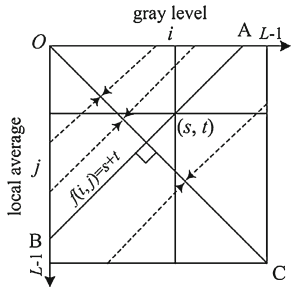
\includegraphics[width=\textwidth]{../../Semestre5/VA_Practicas/Otsu2D/Entrega/metodo1.png}
\end{figure}
\end{columns}
\end{frame}

\begin{frame}
\frametitle{Otsu}
Ahora clasificamos mediante Otsu las $2L-1$ rectas.\\
Buscamos maximizar la varianza entre las dos regiones $$Z(r)= \omega_0(\mu_0-\mu_T)^2+\omega_1(\mu_1-\mu_T)^2$$
Donde $\omega$ es la probabilidad de pertenencia a la clase $$\omega_0=\sum_{r=0}^rp_r\ ,\omega_1=\sum_{r=z+1}^{2L-1}p_r$$
Y $\mu$ es la media de cada clase y $\mu_{T}$ la total
$$ \mu_0 = \frac{\sum_{r=0}^zrp_r}{\sum_{r=0}^zp_r}\ , \mu_1 = \frac{\sum_{r=z+1}^{2L-1}rp_r}{\sum_{r=z+1}^{2L-1}p_r}\ , \mu_T = \frac{\sum_{r=0}^{2L-1}rp_r}{\sum_{r=0}^{2L-1}p_r}$$
\end{frame}

\begin{frame}
\frametitle{Otsu}
En clase lo vimos como 
$$\sigma_B^2=P_1(m_1-m_G)^2+P_2(m_2-m_G)^2=P_1P_2(m_1-m_2)^2$$
Es lo mismo.
$$Z(r)= \omega_0(\mu_0-\mu_T)^2+\omega_1(\mu_1-\mu_T)^2$$
\end{frame}

%------------------------------------------------
\section{Implementación}
%------------------------------------------------

\begin{frame}[fragile]
El cálculo del Histograma:
\begin{lstlisting}
hist2d = zeros(256, 256);   
for row = 1 : rows
    for column = 1 : columns	
        index1 = im(row, column);
        index2 = media(row, column);
        hist2d(index1+1, index2+1) = hist2d(index1+1, index2+1) + 1;
    end
end
hist2dp = double(hist2d)/256^2;
\end{lstlisting}

\end{frame}

\begin{frame}[fragile]
Calculando la suma de los valores de cada recta:
\begin{lstlisting}
sr = zeros(511,1);
for i = 1:256
   for j = 1:i
       sr(i) = sr(i) + hist2dp(j,i+1-j);
       sr(512-i)= sr(512-i) + hist2dp(257-j,256-i+j);
   end
end  
\end{lstlisting}

\end{frame}

\begin{frame}[fragile]
Aplicando la segmentación
\begin{lstlisting}
if kmax < 257
    segim = false(rows,columns);
    for i = 1:kmax
        segim = segim | (im<i & media<(kmax-i));
    end
else % creo que es incorrecta
    segim = true(rows,columns);
    for i = 1:(512-kmax)
        segim = segim & (im<=(257-i) & media<=(kmax-256+i));
    end
end
\end{lstlisting}

\end{frame}

\begin{frame}
\begin{columns}[t]
\column{.45\textwidth} % Left column and width
\begin{figure}
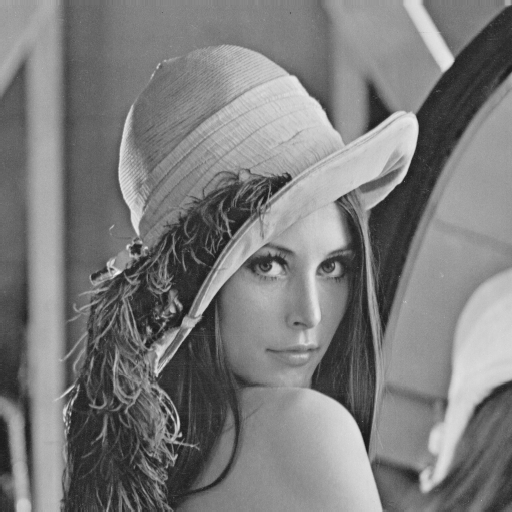
\includegraphics[width=\textwidth]{../../Semestre5/VA_Practicas/Otsu2D/Entrega/lena512.png}
\caption{lena512 original}
\end{figure}

\column{.45\textwidth} % Right column and width
\begin{figure}
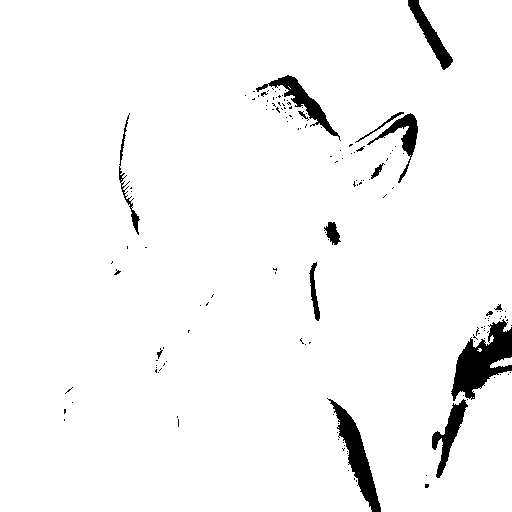
\includegraphics[width=\textwidth]{../../Semestre5/VA_Practicas/Otsu2D/Entrega/seg_lena512.png}
\caption{Segmentación errónea}
\end{figure}

\end{columns}
\end{frame}

%------------------------------------------------
\section{Bibliografía}
%------------------------------------------------
\begin{frame}
\frametitle{Bibliografía}
\footnotesize{
\begin{thebibliography}{99} % Beamer does not support BibTeX so references must be inserted manually as below
\bibitem[Referencia 1]{p1} Fangyan Nie , Yonglin Wang, Meisen Pan, Guanghan Peng, Pingfeng Zhang (2012)
\newblock Two-dimensional extension of variance-based thresholding for image segmentation
\newblock \emph{Multidim Syst Sign Process} 24, 485 -- 501.
\bibitem[Referencia 2]{p1} Puthipong Sthitpattanapongsa and Thitiwan Srinark (2011)
\newblock A Two-stage Otsu’s Thresholding Based Method on a 2D Histogram
\newblock \emph{2011 IEEE International Conference on Intelligent Computer Communication and Processing (ICCP)}  345 -- 348.
\end{thebibliography}
}
\end{frame}


\begin{frame}
\Huge{\centerline{Preguntas y Comentarios}}
\end{frame}

%----------------------------------------------------------------------------------------

\end{document} 